\documentclass[10pt]{article}
\usepackage[T1]{fontenc}\usepackage{lmodern,amsmath,amssymb,graphicx,hyperref}
\usepackage[margin=.75in]{geometry}
\setlength{\parindent}{0pt}\setlength{\parskip}{7pt}
\begin{document}
\begin{center}{\Large Charged creation of rescaled scalar entries}\\[4pt]
Local continuation --- 16 November 2026\end{center}
\textbf{Actual input identity.} Keep the original creation truncation $k$
and moment label $(r,b)$. Let $g=q_i$ for odd $b$, and zero for even $b$,
where $q_i=\min\{2,u-i-1\}$. Existing cleared-representation constructors
build the scalar-rescaled, same-$k$ trimmed right entry. Its integer
numerator is \emph{exactly the old numerator}; its positive denominator is
\[
 D'=D2^g,\qquad E'=v_2(D')=E+g,\qquad
 \operatorname{oddPart}(D')=\operatorname{oddPart}(D).
\]
The original polynomial trim commutes with scalar multiplication via the
existing power-series truncation law. Actual right integrality follows
from the retained-chart content result, including positive-anchor zeros
[pcc:unverified].

\textbf{Constructed scalar word.} The executable denominator uses the
original packed scalar denominator times $2^g$; proof-side polynomial
representations establish equality but are not execution callbacks.
The existing numerator-word constructor evaluates the same old $k$ and
label at width
\[
 W=p_c+E+g.
\]
The existing finite extractor drops exactly $E+g$ low bits and inverts the
actual odd denominator part. The resulting word has exactly the canonical
reduction of the rescaled coefficient at creation precision $p_c$.
The statement includes all $p_c$, signed and zero integer numerators;
zero gain is included without a special favorable premise
[pcc:unverified].

\textbf{Emitted arithmetic is charged.} With the existing bound $N_*$ on
the actual approximation expression and
$C(W,h,z)=10(W+1)^2(hz+1)^2$, the actual emitted XOR/AND/OR trace satisfies
\[
 \#\mathrm{events}\le C(W,b+1,\ell+1)N_*+6W+5W^2
                   +10p_c^3+16p_c^2.
\]
This uses the enlarged $W$, rather than the old width. It counts the named
arithmetic events, not all hardware gates or full bit runtime. Scalar,
AST, denominator, bit preparation, allocation, control, indexing, traces
and memory are not free [pcc:unverified].

\textbf{Immutable scalar reuse.} The actual creation word is stored in
the existing scalar frozen object. At later $P\ge p_c$, the existing lift
pads high zeros and preserves its canonical creation integer; it does not
reevaluate the formula at $P$. This is a scalar coordinate contract, not a
binding of the original extension basis or full packet descriptions
[pcc:unverified].

\textbf{Precision control.} For $m>0,d>1$, no arbitrary function of a
residue modulo $md$ computes $n/d$ modulo the same modulus for every
natural $n$ divisible by $d$. Inputs zero and $md$ have equal residues;
quotients zero and $m$ have different residues. This generic control
rejects an in-place division shortcut. It is not an information lower
bound for the actual chart family [pcc:unverified].
\newpage
\begin{center}{\Large Evidence and the next mode obligation}\end{center}
\begin{center}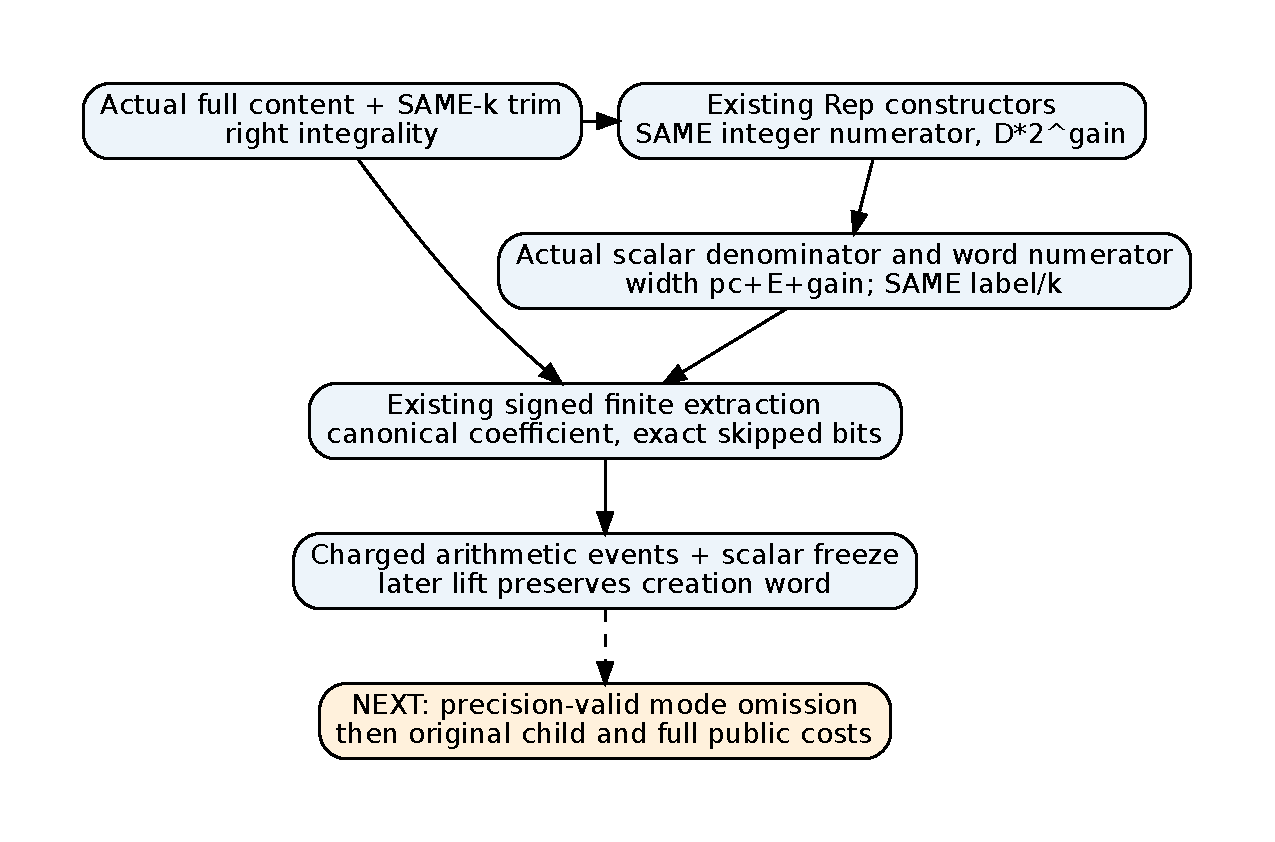
\includegraphics[width=\linewidth,height=2.25in,keepaspectratio]{rescaled-creation-dependencies-001.pdf}\end{center}
\textbf{Accepted local evidence.} Readonly qualifier117 has497 named source
statements including485, with12 new denominator, numerator, trim and width
contracts. Readonly119 has504 including497, with seven new actual scalar
value, emitted-event, skipped-bit and frozen-lift contracts. Both exit zero
without warnings or sorryAx; central printed dependencies are standard.
Receipts065 and066 bind their exact pre-call source hashes, raw outputs
and exits [pcc:unverified].

\textbf{Generic owner control.} CryptoLean commit5613064 contains the one
same-residue quotient control. A separately copied readonly qualifier and
identical owner module both pass without warnings; the existing pinned
import-based auditor reports one theorem, zero failing and zero trusted.
Receipt064 pins this scoped evidence. All new records remain unsigned and
defaultnot\_covered. These prototypes are outside shared Transport53/57/fresh
coverage; the scoped owner audit does not cover the full study. Consumer
dependency pins are unchanged and the owner overlay is explicit
[pcc:unverified].

\textbf{Sources reused as stated.} The denominator laws directly apply
Mathlib's natural valuation and maximal-power-removal laws. Rational inverse
numerator/denominator laws establish the exact old numerator. Existing
representation constructors, power-series constant truncation, word numerator,
signed finite extraction and frozen-word lifting supply the remaining
interfaces. No Newton, adder, convolution or valuation induction was
reimplemented. KB access was unavailable; exact primary sources were used
[pcc:unverified].

\textbf{Failures preserved.} Owner qualifier001 had a wrong tactic-module
import;002 uses the existing module. Study116 had incorrect owning namespaces
and a power-lemma argument. Study118 omitted the cost function's owner
namespace. Every rejected source, immutable qualifier, pre-call hash, raw
output and exit is retained. No linter, opacity, trust or resource override
was used [pcc:unverified].

\textbf{Next discriminating action.} Protocol019 tests whether columns
whose new left weight already reaches $p_c$ can be omitted while preserving
the actual residual, then counts the parity-dependent survivors. All
$2^u k$ labels remain charged until that theorem is established. Every
zeroth mode must remain as an exact control. No rank, density or runtime
conclusion follows from active counts alone [pcc:unverified].

Original packet and extension representation, child entry and edge
interfaces, degree and recursion, public elliptic relations, finding and
scalar extraction, retries and the full cold expected bit cost remain open.
The protected remote ledger blocks publication; it does not stop this
independent mathematics. No native, paid, timing, scaling or attack campaign
was run [pcc:unverified].
\end{document}
